
%% ECSE 420 -- Project proposal

%
\documentclass[conference]{IEEEtran}
%
% If IEEEtran.cls has not been installed into the LaTeX system files,
% manually specify the path to it like:
% \documentclass[conference]{../sty/IEEEtran}


%My packages
\usepackage{graphicx,dblfloatfix}
\graphicspath{{./figures/}}
\usepackage[xetex,colorlinks=true,urlcolor = black, 
linkcolor=black,citecolor=black]{hyperref}


% correct bad hyphenation here
\hyphenation{op-tical net-works semi-conduc-tor}


\begin{document}

% paper title
% can use linebreaks \\ within to get better formatting as desired
\title{ECSE 548 - Project Status Report:\\ 8-bit Booth Multiplier}
%\author{\IEEEauthorblockN{Marco Kassis\IEEEauthorrefmark{1},
%Aryan Mojtahedi\IEEEauthorrefmark{1},
%Dimitrios Stamoulis\IEEEauthorrefmark{1} and
%Louis-Charles Trudeau\IEEEauthorrefmark{1}\IEEEauthorrefmark{2}}
%\IEEEauthorblockA{\IEEEauthorrefmark{1}McGill University, Montreal, Canada ~~~~~ \IEEEauthorrefmark{2}Ecole de technologie superieure, Montreal, Canada}
\author{\IEEEauthorblockN{Marco Kassis,
Aryan Mojtahedi,
Dimitrios Stamoulis and
Louis-Charles Trudeau}
\IEEEauthorblockA{Department of Electrical and Computer Engineering, McGill University, Montreal, Canada}

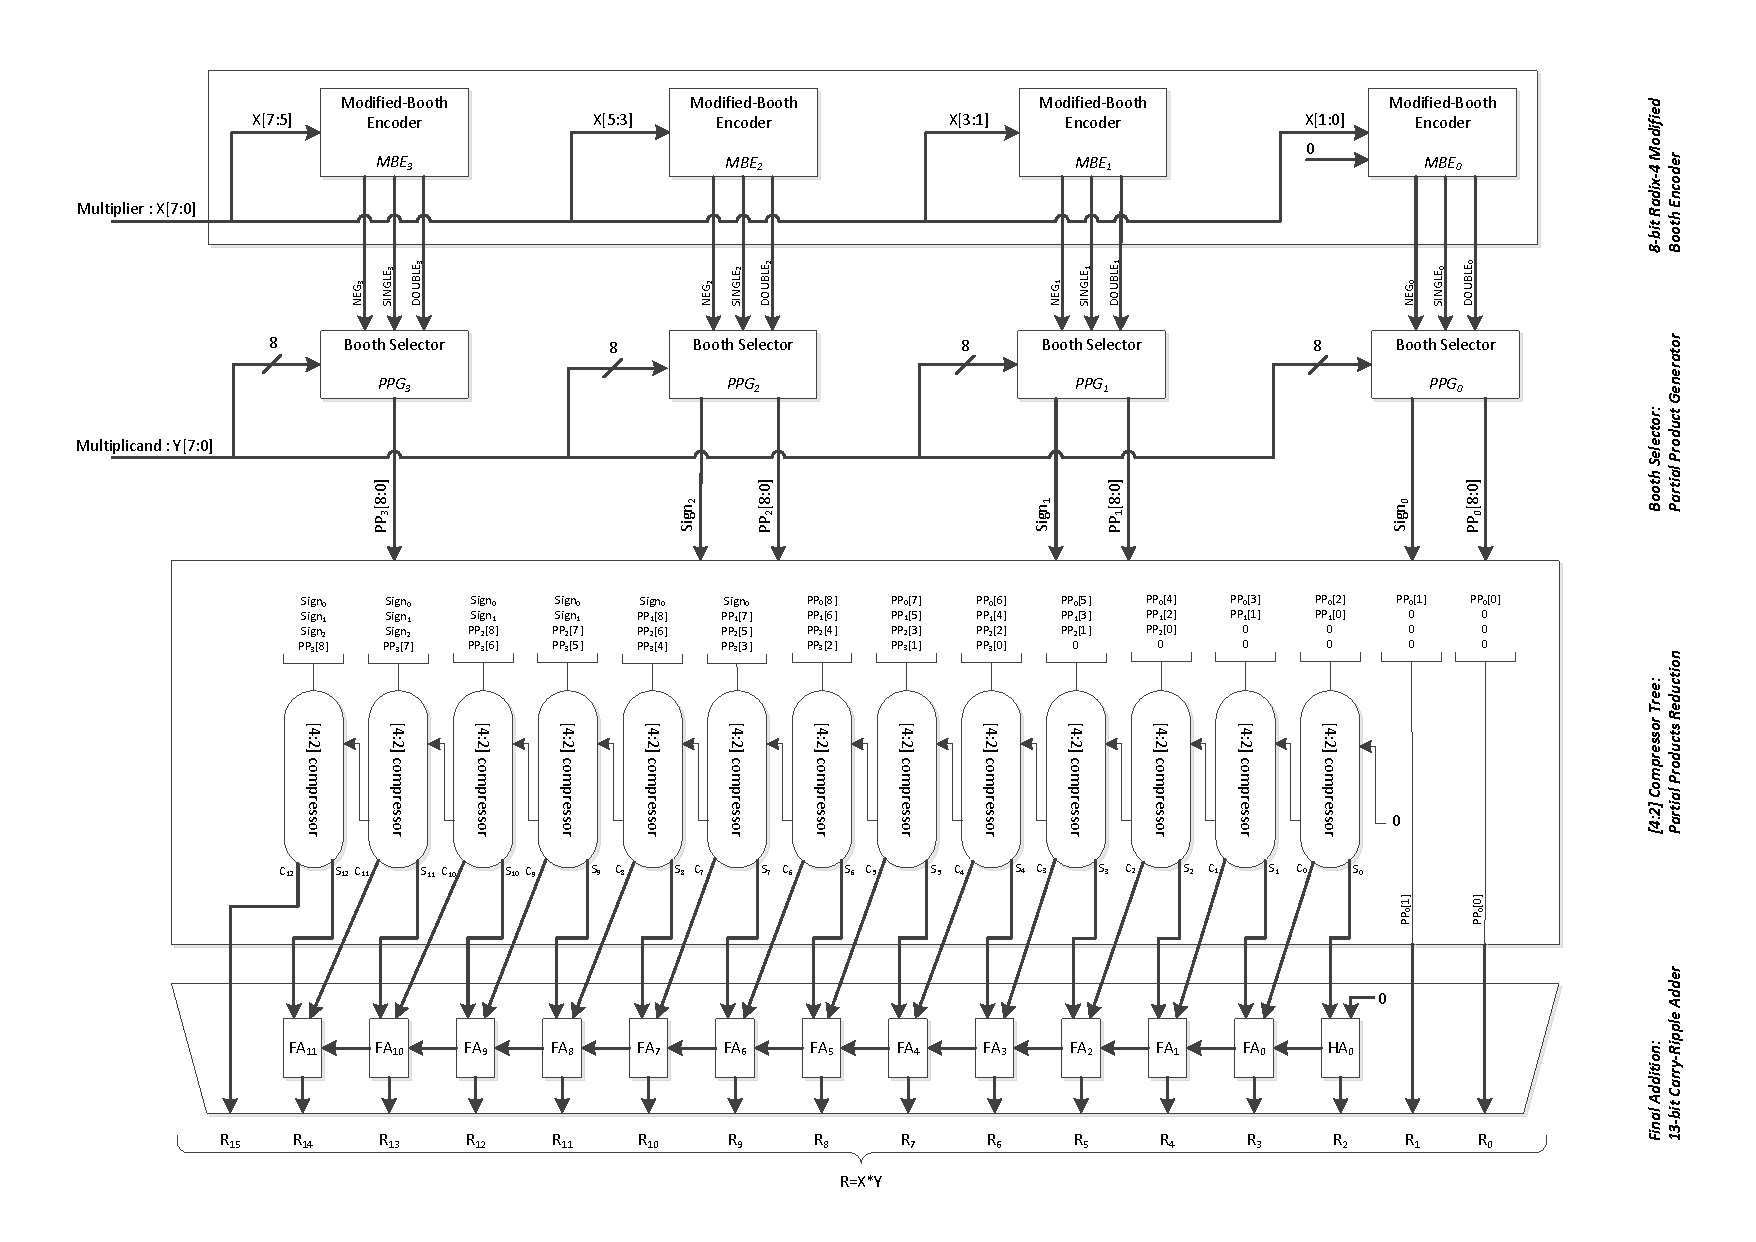
\includegraphics[height=0.3\textheight, width=0.7\linewidth]{BoothTopLevel.pdf}
\\Fig. 1. Top-Level Design\\~\\
}

% make the title area
\maketitle
\IEEEpeerreviewmaketitle

\section{Introduction}
\IEEEPARstart{T}{he} current document is the 
submitted Project Status Report written in 
\LaTeX ~ IEEE format. The steps of
our design plan were completed under \textbf{version control}.
The proper GitHub Repo has been created \cite{git}. 


\section{Completed Deliverables\cite{gitDel}}
Design part:
\begin{itemize}
\item \textbf{Exploration of the Modified Booth algorithm:}
The theoretical background was studied based on 
related online material and our textbook\cite{tb}.

\item \textbf{Application in the 8-bit multiplier case:}
Having the functionality of our design 
well defined, we proceed with the Top-Level design 
of our 8-bit Booth Multiplier.
The outcome of such an exploration is presented
in Figure 1.

\end{itemize}

Implementation part:
\begin{itemize}
\item \textbf{Circuit schematics:}
We first implemented 
any required basic logic gates (e.g optimized 
XNOR gate) and added them to the
\texttt{muddlib07.jelib} Electic library.
The building blocks of our design
(e.g Booth Encoder, Partial Product Generator etc)
were created and added to the
\texttt{wordlib8.jelib} Electic library.
The top-level schematic was added to 
the \texttt{mips8.jelib} Electic library.


\item \textbf{Verified correctness of modules:}
All the designed schematics they do pass the 
DRC check using Electric.

\item \textbf{Complete testbenching procedure}
The proper Verilog decks were generated using
Electic. All the individual submodules and the
main building blocks were tested using the 
appropriate Modelsim testbenches.

\end{itemize}




\section{Encountered Issues}

No issues were encountered
in carrying out	the aforementioned 
deliverables. The implementation was
straight-forward and the verification
of their correctness was completed with
the proper DRC checks and Modelsim 
testbenches.

\section{Changes in the implementation plan}

No need for any changes in the implementation
procedure. On the contrary, we are one week ahead
based on our initial implementation plan and we
have already started studying the
layout (area minimization, transistor sizing etc)


%\section{Conclusion}
%The conclusion goes here.


% conference papers do not normally have an appendix
% use section* for acknowledgement
%\section*{Acknowledgment}
%The authors would like to thank...


% references section
\begin{thebibliography}{1}

\bibitem{git}
GitHub - Project Repository,
\href{https://github.com/dstamoulis/anonymous-dinosaurs}{https://github.com/dstamoulis/anonymous-dinosaurs}.



\bibitem{gitDel}
GitRepo - Project Status Report,
\href{https://github.com/dstamoulis/anonymous-dinosaurs/tree/master/ProjectStatusReport}{https://github.com/dstamoulis/anonymous-dinosaurs/tree/master/ProjectStatusReport}.

\bibitem{tb}
Weste and Harris, \emph{CMOS VLSI Design}, $4^{th}$ edition, Addison-Wesley, 2011.	



\end{thebibliography}




% that's all folks
\end{document}

